\input{header.tex}

\begin{document}

\lecture{ 33 --- File System Implementation }{\term}{Jeff Zarnett}

\section*{File System Implementation}
Now it is time to go behind the scenes of how the file system lives up to the interface we have just finished discussing. The implementation is somewhat complicated, and to keep the size of the problem manageable we will worry about storing files on hard disks. Hard disks themselves make a good choice for this: they are sufficiently large and sufficiently cheap, to start with, to store the data that we want to store. We can read an arbitrary part of the disk (unlike a tape). Finally, we can write to the same part of disk as many times as we want (disks don't, at least on the time frames that we are concerned about, wear out). Recall also that disks operate on blocks which, in their physical representation, comprise one or more sectors.

Let us take a look at the layers of the file system's design, from~\cite{osc}. As we descend down the list we will get closer to the hardware and less abstraction.

\paragraph{The File System.} The file system user interface is intended for the convenience of the user and for application programmers. This is the level we have just examined in the previous topic; the more interesting part is what happens when we need to fulfill the promises that the file system makes.

\paragraph{I/O Control.} At the I/O control level, we are dealing with device drivers and interrupt handlers to transfer data. The inputs are fairly high-level commands, along the lines of ``read block 1234''. Its outputs are hardware specific-instructions to the hardware controller. Usually this is by writing bit patterns in the I/O controller memory.

\paragraph{Basic File System.} Despite the awful name, this is the level at which we start to deal with physical blocks on the disk. A physical block is identified by its numerical physical address: drive 0, cylinder 12, track 7, sector 1. This layer is also responsible for buffers and caches that are used to hold various commonly-accessed regions (e.g., the temporary directory). Yes, caching and buffers can appear in the hard disk as well, with performance improvements traded off against the risk of data loss if power is suddenly cut.

\paragraph{File Organization Module.} This module is aware of files and their logical and physical blocks. This translates a logical block address to a physical block address, keeps track of free space (unallocated blocks).

\paragraph{The Logical File System.} This last level is for managing metadata: file system structure, directory structure, and maintaining the file structure. File data is maintained in a \textit{file control block} (FCB). The UNIX term for this is \textit{inode} and it is the place where file info is stores: ownership, permissions, locations of the file contents.

\subsection*{Disk Organization}

Although there are a million different file systems (UFS, HFS+, ZFS, NTFS, ext3, FAT32...) that are all significantly different, there are some general principles that we can examine. A file system will need to keep track of the total number of blocks, the number and locations of free blocks, the directory structure, and the files themselves.

On at least one disk somewhere in the system, there will need to be some information about how to boot up the operating system. Not every disk has the operating system on it, but if there is an OS the boot loader is usually put in the first block. When the power button is pressed on the case, the BIOS starts up and transfers control to whatever is found at that first block (which is hopefully your boot loader that launches the OS, or gives you the option of which OS to start).

Disks may be split, logically, into several different areas, or \textit{partitions}. Accordingly, there will be a partition table (sometimes called the superblock or master file table) that indicates what part of the disk belongs to which partition. In the Windows world we often see the whole disk is in one logical partition (the C: drive, for example, taking the whole primary disk). In Linux we often see the disk divided up to have partitions for different things: temporary/swap directory, home directories, boot partition, et cetera...

There are several structures that are likely to be in memory for performance reasons~\cite{osc}:

\begin{enumerate}
	\item \textbf{Mount Table}: Information about each mounted volume (disk/partition).
	\item \textbf{Cache}: Directory info for recently accessed directories.
	\item \textbf{Global Open File Table}: Copy of the FCB for each open file.
	\item \textbf{Process Open File Table}: References to the global open file table, sorted by process.
	\item \textbf{Buffers}: places where data read from or to be written to disk resides after or before the actual disk operation.
\end{enumerate}

Creating a new file is the job of the logical file system: allocation of a new FCB (or re-use of an existing free FCB). A typical FCB might look like this:

\begin{center}
	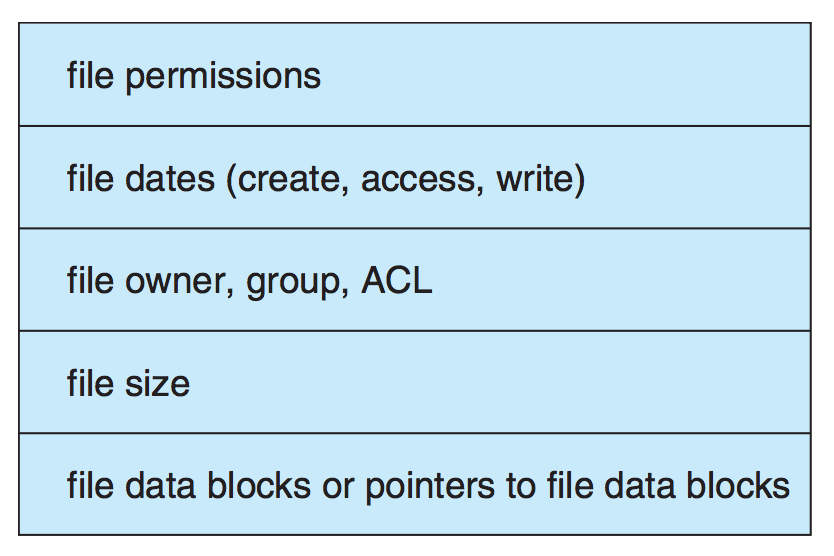
\includegraphics[width=0.4\textwidth]{images/fcb.png}\\
	File Control Block (FCB) example~\cite{osc}.
\end{center}

If a user (application) actually wants to make use of a file, the open system call is needed. Open operates on names, the user comprehensible version. The file system must then check the global open file table to see if the file is already open somewhere in the system. If so, if that file is opened for exclusive access, then the open routine returns with an error. If it is open but for non-exclusive access, then there is no need to search for the file or retrieve it by directory; we just make another reference in the process open file table. If the file is not already open, then it needs to be retrieved; once the file is found, the FCB is copied into the global open file table and the appropriate reference is added to the process table~\cite{osc}.

The process open file table can contain some additional information, like the next section to read or write, the access mode when the file is open, and so on. The open system call returns a pointer to the file table and this is the route through which the application performs all file operations. In UNIX this reference is called a \textit{file descriptor}; in Windows it is called a \textit{file handle}~\cite{osc}.

The opposite operation to opening a file is obviously to close it. When a process closes a file, the entry from the process open file table can be removed. If this is the last reference to the file a process has, then the file can also be removed from the global open file table. Metadata may be updated on close.

The diagram below shows how a file is opened and how a read takes place:

\begin{center}
	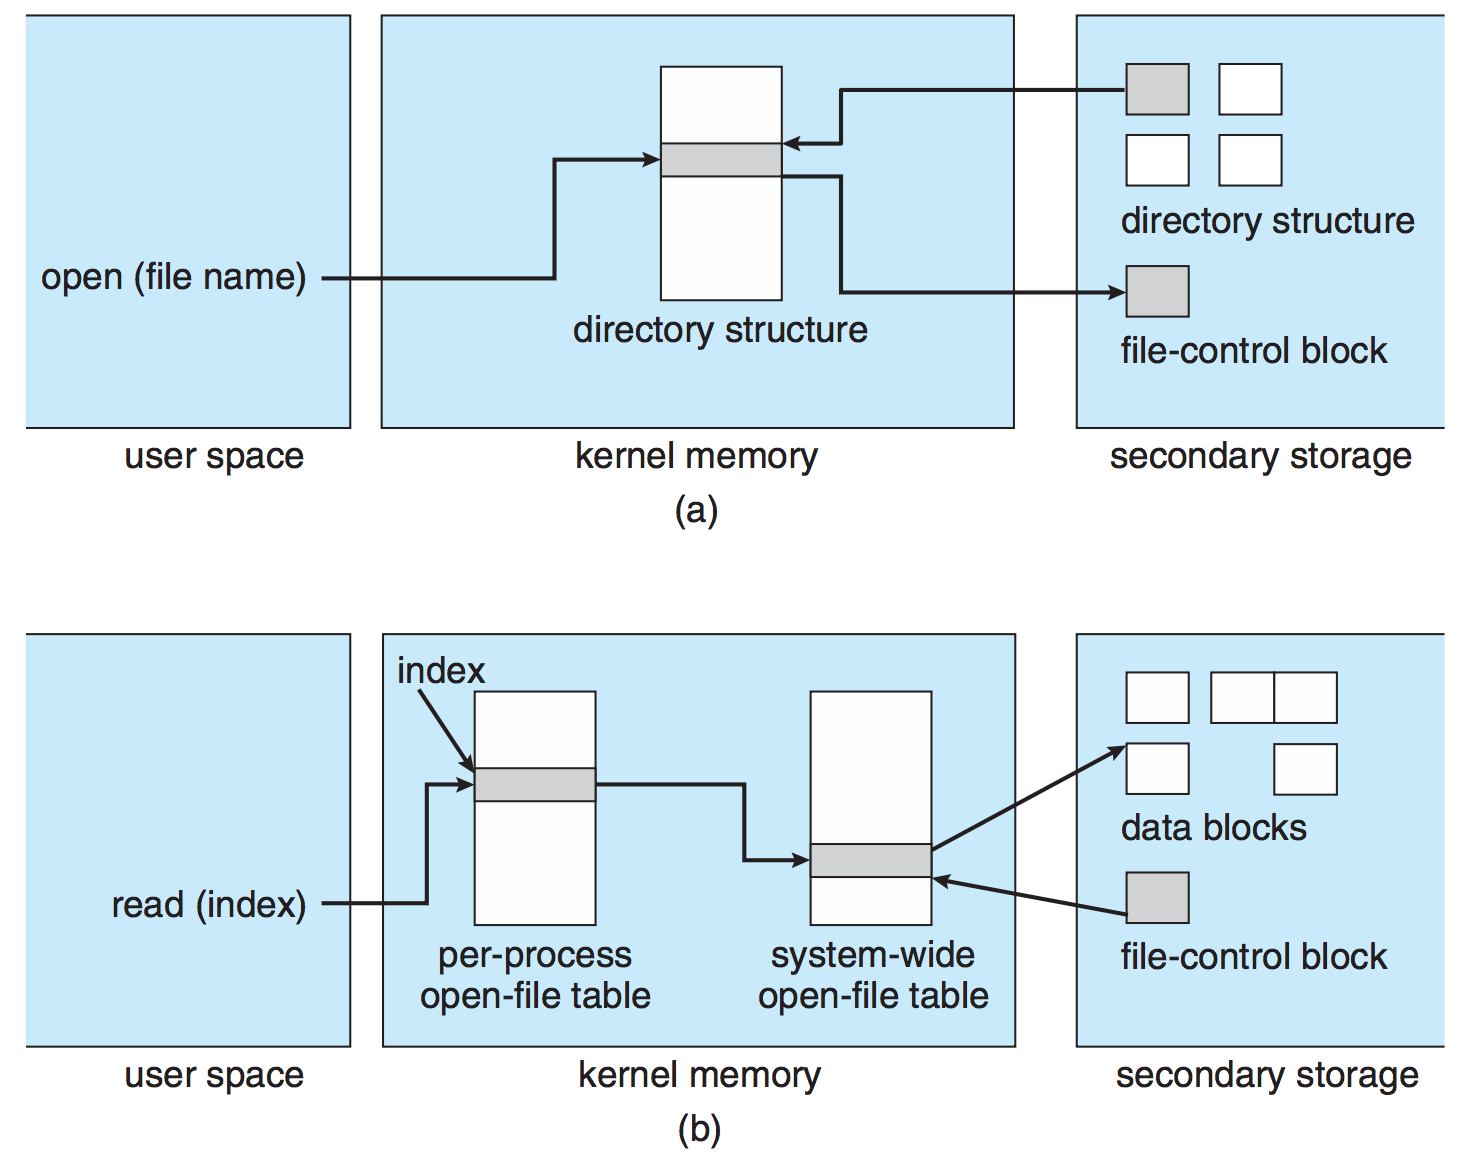
\includegraphics[width=0.75\textwidth]{images/file-system-structures.png}\\
	File System Structures for (a) file open and (b) file read~\cite{osc}.
\end{center}

\subsection*{Virtual File System}

\subsection*{Directory Implementation}

\subsection*{Allocation Methods}




\input{bibliography.tex}

\end{document}